\documentclass[a4paper]{book}
\usepackage{makeidx}
\usepackage{graphicx}
\usepackage{multicol}
\usepackage{float}
\usepackage{listings}
\usepackage{color}
\usepackage{textcomp}
\usepackage{alltt}
\usepackage{times}
\usepackage{ifpdf}
\ifpdf
\usepackage[pdftex,
            pagebackref=true,
            colorlinks=true,
            linkcolor=blue,
            unicode
           ]{hyperref}
\else
\usepackage[ps2pdf,
            pagebackref=true,
            colorlinks=true,
            linkcolor=blue,
            unicode
           ]{hyperref}
\usepackage{pspicture}
\fi
\usepackage[utf8]{inputenc}
\usepackage{doxygen}
\lstset{language=C++,inputencoding=utf8,basicstyle=\footnotesize,breaklines=true,breakatwhitespace=true,tabsize=4,numbers=left }
\makeindex
\setcounter{tocdepth}{3}
\renewcommand{\footrulewidth}{0.4pt}
\begin{document}
\hypersetup{pageanchor=false}
\begin{titlepage}
\vspace*{7cm}
\begin{center}
{\Large Entwurf und Implementierung einer Schnittstelle zur Kopplung von virtuellen Avionik-\/Systemen \\[1ex]\large WS 2012/2013 }\\
\vspace*{1cm}
{\large Generated by Doxygen 1.7.1}\\
\vspace*{0.5cm}
{\small Sat Feb 23 2013 22:02:49}\\
\end{center}
\end{titlepage}
\clearemptydoublepage
\pagenumbering{roman}
\tableofcontents
\clearemptydoublepage
\pagenumbering{arabic}
\hypersetup{pageanchor=true}
\chapter{Class Index}
\section{Class List}
Here are the classes, structs, unions and interfaces with brief descriptions:\begin{DoxyCompactList}
\item\contentsline{section}{\hyperlink{class_example_c_p_p_federate}{ExampleCPPFederate} }{\pageref{class_example_c_p_p_federate}}{}
\item\contentsline{section}{\hyperlink{class_example_fed_amb}{ExampleFedAmb} }{\pageref{class_example_fed_amb}}{}
\end{DoxyCompactList}

\chapter{File Index}
\section{File List}
Here is a list of all documented files with brief descriptions:\begin{DoxyCompactList}
\item\contentsline{section}{\hyperlink{_example_c_p_p_federate_8cpp}{ExampleCPPFederate.cpp} }{\pageref{_example_c_p_p_federate_8cpp}}{}
\item\contentsline{section}{\hyperlink{_example_c_p_p_federate_8h}{ExampleCPPFederate.h} }{\pageref{_example_c_p_p_federate_8h}}{}
\item\contentsline{section}{\hyperlink{_example_fed_amb_8cpp}{ExampleFedAmb.cpp} }{\pageref{_example_fed_amb_8cpp}}{}
\item\contentsline{section}{\hyperlink{_example_fed_amb_8h}{ExampleFedAmb.h} }{\pageref{_example_fed_amb_8h}}{}
\item\contentsline{section}{\hyperlink{main_8cpp}{main.cpp} }{\pageref{main_8cpp}}{}
\end{DoxyCompactList}

\chapter{Class Documentation}
\hypertarget{class_example_c_p_p_federate}{
\section{ExampleCPPFederate Class Reference}
\label{class_example_c_p_p_federate}\index{ExampleCPPFederate@{ExampleCPPFederate}}
}


{\ttfamily \#include $<$ExampleCPPFederate.h$>$}



Collaboration diagram for ExampleCPPFederate:\nopagebreak
\begin{figure}[H]
\begin{center}
\leavevmode
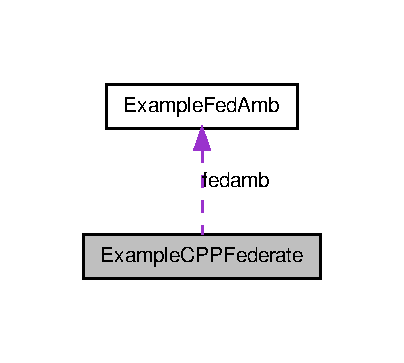
\includegraphics[width=194pt]{class_example_c_p_p_federate__coll__graph}
\end{center}
\end{figure}
\subsection*{Public Member Functions}
\begin{DoxyCompactItemize}
\item 
\hypertarget{class_example_c_p_p_federate_abf1c885a01fb942a1120f8ea1b93b511}{
\hyperlink{class_example_c_p_p_federate_abf1c885a01fb942a1120f8ea1b93b511}{ExampleCPPFederate} ()}
\label{class_example_c_p_p_federate_abf1c885a01fb942a1120f8ea1b93b511}

\begin{DoxyCompactList}\small\item\em Constructor. \item\end{DoxyCompactList}\item 
\hypertarget{class_example_c_p_p_federate_a7b5810837c8fd7e5dadcf8ff84bfb6ec}{
virtual \hyperlink{class_example_c_p_p_federate_a7b5810837c8fd7e5dadcf8ff84bfb6ec}{$\sim$ExampleCPPFederate} ()}
\label{class_example_c_p_p_federate_a7b5810837c8fd7e5dadcf8ff84bfb6ec}

\begin{DoxyCompactList}\small\item\em Destructor. \item\end{DoxyCompactList}\item 
void \hyperlink{class_example_c_p_p_federate_a1b8a60b635555f1723eab0bde159f5f5}{runFederate} (std::string federateName, std::string fom, std::string address)
\begin{DoxyCompactList}\small\item\em Main Simulation Method. \item\end{DoxyCompactList}\end{DoxyCompactItemize}
\subsection*{Public Attributes}
\begin{DoxyCompactItemize}
\item 
std::auto\_\-ptr$<$ rti1516::RTIambassador $>$ \hyperlink{class_example_c_p_p_federate_ac4d4b4416ce7ab50284c6a3c2deecaa4}{rtiamb}
\item 
\hyperlink{class_example_fed_amb}{ExampleFedAmb} $\ast$ \hyperlink{class_example_c_p_p_federate_acc3635b1ef16e90ac4fad62150808f1e}{fedamb}
\end{DoxyCompactItemize}
\subsection*{Private Member Functions}
\begin{DoxyCompactItemize}
\item 
std::wstring \hyperlink{class_example_c_p_p_federate_af5e9565fdea92cdee1cd27bbe7ad74ce}{convertStringToWstring} (const std::string \&str)
\item 
rti1516::VariableLengthData \hyperlink{class_example_c_p_p_federate_aaf7e26b8a397f6d87ae2c27326cde893}{toVariableLengthData} (const char $\ast$s)
\item 
void \hyperlink{class_example_c_p_p_federate_a1fde2254c348389efc4cd894e03fce87}{initializeHandles} ()
\item 
void \hyperlink{class_example_c_p_p_federate_a8a6fa5956cc241097e15385ca2da433f}{waitForUser} ()
\item 
void \hyperlink{class_example_c_p_p_federate_a5184192fe0adb7b0259151dfbd8245e3}{enableTimePolicy} ()
\item 
void \hyperlink{class_example_c_p_p_federate_a57413d733e33b493abd929a7e46ff3dc}{publishAndSubscribe} ()
\item 
ObjectInstanceHandle \hyperlink{class_example_c_p_p_federate_afe34dcca7757b66ebbf9d2dea37e3440}{registerObject} ()
\item 
void \hyperlink{class_example_c_p_p_federate_ad2d6193d942e59a2cf5ee05531962967}{updateAttributeValues} (ObjectInstanceHandle objectHandle)
\item 
void \hyperlink{class_example_c_p_p_federate_a60bb15d2fc7a3437c13e8d8e09df8a1a}{sendInteraction} ()
\item 
void \hyperlink{class_example_c_p_p_federate_adfbfb26a2eeac388c3f5c2f68844ca13}{advanceTime} (double timestep)
\item 
void \hyperlink{class_example_c_p_p_federate_a7b6dcb57aea95b30d384187b551e03ae}{deleteObject} (ObjectInstanceHandle objectHandle)
\item 
\hypertarget{class_example_c_p_p_federate_a04d499d8cab5b555440199bc12524d65}{
double {\bfseries getLbts} ()}
\label{class_example_c_p_p_federate_a04d499d8cab5b555440199bc12524d65}

\end{DoxyCompactItemize}
\subsection*{Private Attributes}
\begin{DoxyCompactItemize}
\item 
\hypertarget{class_example_c_p_p_federate_a0a0ce0cd597402f43b466766a3bd80a3}{
ObjectClassHandle \hyperlink{class_example_c_p_p_federate_a0a0ce0cd597402f43b466766a3bd80a3}{aHandle}}
\label{class_example_c_p_p_federate_a0a0ce0cd597402f43b466766a3bd80a3}

\begin{DoxyCompactList}\small\item\em fom handles \item\end{DoxyCompactList}\item 
\hypertarget{class_example_c_p_p_federate_a0aa9a8fe9e608c94ed28e6ba8f9cec40}{
AttributeHandle {\bfseries aaHandle}}
\label{class_example_c_p_p_federate_a0aa9a8fe9e608c94ed28e6ba8f9cec40}

\item 
\hypertarget{class_example_c_p_p_federate_afce0ad65479022ee261dc269d6869863}{
AttributeHandle {\bfseries abHandle}}
\label{class_example_c_p_p_federate_afce0ad65479022ee261dc269d6869863}

\item 
\hypertarget{class_example_c_p_p_federate_aa36baca43769fc83d21223d4e1b23dda}{
AttributeHandle {\bfseries acHandle}}
\label{class_example_c_p_p_federate_aa36baca43769fc83d21223d4e1b23dda}

\item 
\hypertarget{class_example_c_p_p_federate_a35fb74ee07c623089c1bf3a3e84cf5da}{
InteractionClassHandle {\bfseries xHandle}}
\label{class_example_c_p_p_federate_a35fb74ee07c623089c1bf3a3e84cf5da}

\item 
\hypertarget{class_example_c_p_p_federate_ae54b6dcb8713459480b0d2983d41d2cc}{
ParameterHandle {\bfseries xaHandle}}
\label{class_example_c_p_p_federate_ae54b6dcb8713459480b0d2983d41d2cc}

\item 
\hypertarget{class_example_c_p_p_federate_a537ff0d9190c2df3fdc526c0b51e0069}{
ParameterHandle {\bfseries xbHandle}}
\label{class_example_c_p_p_federate_a537ff0d9190c2df3fdc526c0b51e0069}

\end{DoxyCompactItemize}


\subsection{Detailed Description}
Example Federate implementation 

\subsection{Member Function Documentation}
\hypertarget{class_example_c_p_p_federate_adfbfb26a2eeac388c3f5c2f68844ca13}{
\index{ExampleCPPFederate@{ExampleCPPFederate}!advanceTime@{advanceTime}}
\index{advanceTime@{advanceTime}!ExampleCPPFederate@{ExampleCPPFederate}}
\subsubsection[{advanceTime}]{\setlength{\rightskip}{0pt plus 5cm}void ExampleCPPFederate::advanceTime (
\begin{DoxyParamCaption}
\item[{double}]{ timestep}
\end{DoxyParamCaption}
)\hspace{0.3cm}{\ttfamily  \mbox{[}private\mbox{]}}}}
\label{class_example_c_p_p_federate_adfbfb26a2eeac388c3f5c2f68844ca13}
This method will request a time advance to the current time, plus the given timestep. It will then wait until a notification of the time advance grant has been received. 

request the advance

wait for the time advance to be granted. ticking will tell the LRC to start delivering callbacks to the federate 

\hypertarget{class_example_c_p_p_federate_af5e9565fdea92cdee1cd27bbe7ad74ce}{
\index{ExampleCPPFederate@{ExampleCPPFederate}!convertStringToWstring@{convertStringToWstring}}
\index{convertStringToWstring@{convertStringToWstring}!ExampleCPPFederate@{ExampleCPPFederate}}
\subsubsection[{convertStringToWstring}]{\setlength{\rightskip}{0pt plus 5cm}std::wstring ExampleCPPFederate::convertStringToWstring (
\begin{DoxyParamCaption}
\item[{const std::string \&}]{ str}
\end{DoxyParamCaption}
)\hspace{0.3cm}{\ttfamily  \mbox{[}private\mbox{]}}}}
\label{class_example_c_p_p_federate_af5e9565fdea92cdee1cd27bbe7ad74ce}
convert normal C++-\/Strings to C++-\/Wstrings Wstrings are used by openrti \hypertarget{class_example_c_p_p_federate_a7b6dcb57aea95b30d384187b551e03ae}{
\index{ExampleCPPFederate@{ExampleCPPFederate}!deleteObject@{deleteObject}}
\index{deleteObject@{deleteObject}!ExampleCPPFederate@{ExampleCPPFederate}}
\subsubsection[{deleteObject}]{\setlength{\rightskip}{0pt plus 5cm}void ExampleCPPFederate::deleteObject (
\begin{DoxyParamCaption}
\item[{ObjectInstanceHandle}]{ objectHandle}
\end{DoxyParamCaption}
)\hspace{0.3cm}{\ttfamily  \mbox{[}private\mbox{]}}}}
\label{class_example_c_p_p_federate_a7b6dcb57aea95b30d384187b551e03ae}
This method will attempt to delete the object instance of the given handle. We can only delete objects we created, or for which we own the privilegeToDelete attribute. \hypertarget{class_example_c_p_p_federate_a5184192fe0adb7b0259151dfbd8245e3}{
\index{ExampleCPPFederate@{ExampleCPPFederate}!enableTimePolicy@{enableTimePolicy}}
\index{enableTimePolicy@{enableTimePolicy}!ExampleCPPFederate@{ExampleCPPFederate}}
\subsubsection[{enableTimePolicy}]{\setlength{\rightskip}{0pt plus 5cm}void ExampleCPPFederate::enableTimePolicy (
\begin{DoxyParamCaption}
{}
\end{DoxyParamCaption}
)\hspace{0.3cm}{\ttfamily  \mbox{[}private\mbox{]}}}}
\label{class_example_c_p_p_federate_a5184192fe0adb7b0259151dfbd8245e3}
This method will attempt to enable the various time related properties for the federate 

enable time regulation

wait for callback

enable time constrained

wait for callback 

\hypertarget{class_example_c_p_p_federate_a1fde2254c348389efc4cd894e03fce87}{
\index{ExampleCPPFederate@{ExampleCPPFederate}!initializeHandles@{initializeHandles}}
\index{initializeHandles@{initializeHandles}!ExampleCPPFederate@{ExampleCPPFederate}}
\subsubsection[{initializeHandles}]{\setlength{\rightskip}{0pt plus 5cm}void ExampleCPPFederate::initializeHandles (
\begin{DoxyParamCaption}
{}
\end{DoxyParamCaption}
)\hspace{0.3cm}{\ttfamily  \mbox{[}private\mbox{]}}}}
\label{class_example_c_p_p_federate_a1fde2254c348389efc4cd894e03fce87}
This method will get all the relevant handle information from the RTIambassador \hypertarget{class_example_c_p_p_federate_a57413d733e33b493abd929a7e46ff3dc}{
\index{ExampleCPPFederate@{ExampleCPPFederate}!publishAndSubscribe@{publishAndSubscribe}}
\index{publishAndSubscribe@{publishAndSubscribe}!ExampleCPPFederate@{ExampleCPPFederate}}
\subsubsection[{publishAndSubscribe}]{\setlength{\rightskip}{0pt plus 5cm}void ExampleCPPFederate::publishAndSubscribe (
\begin{DoxyParamCaption}
{}
\end{DoxyParamCaption}
)\hspace{0.3cm}{\ttfamily  \mbox{[}private\mbox{]}}}}
\label{class_example_c_p_p_federate_a57413d733e33b493abd929a7e46ff3dc}
This method will inform the RTI about the types of data that the federate will be creating, and the types of data we are interested in hearing about as other federates produce it. 

publish all attributes of ObjectRoot.A

before we can register instance of the object class ObjectRoot.A and update the values of the various attributes, we need to tell the RTI that we intend to publish this information\par


package the information into a handle set

do the actual publication

subscribe to all attributes of ObjectRoot.A

we also want to hear about the same sort of information as it is created and altered in other federates, so we need to subscribe to it

publish the interaction class InteractionRoot.X

we want to send interactions of type InteractionRoot.X, so we need to tell the RTI that we're publishing it first. We don't need to inform it of the parameters, only the class, making it much simpler

do the publication

subscribe to the InteractionRoot.X interaction //

we also want to receive other interaction of the same type that are sent out by other federates, so we have to subscribe to it first 

\hypertarget{class_example_c_p_p_federate_afe34dcca7757b66ebbf9d2dea37e3440}{
\index{ExampleCPPFederate@{ExampleCPPFederate}!registerObject@{registerObject}}
\index{registerObject@{registerObject}!ExampleCPPFederate@{ExampleCPPFederate}}
\subsubsection[{registerObject}]{\setlength{\rightskip}{0pt plus 5cm}ObjectInstanceHandle ExampleCPPFederate::registerObject (
\begin{DoxyParamCaption}
{}
\end{DoxyParamCaption}
)\hspace{0.3cm}{\ttfamily  \mbox{[}private\mbox{]}}}}
\label{class_example_c_p_p_federate_afe34dcca7757b66ebbf9d2dea37e3440}
This method will register an instance of the class ObjectRoot.A and will return the federation-\/wide unique handle for that instance. Later in the simulation, we will update the attribute values for this instance \hypertarget{class_example_c_p_p_federate_a1b8a60b635555f1723eab0bde159f5f5}{
\index{ExampleCPPFederate@{ExampleCPPFederate}!runFederate@{runFederate}}
\index{runFederate@{runFederate}!ExampleCPPFederate@{ExampleCPPFederate}}
\subsubsection[{runFederate}]{\setlength{\rightskip}{0pt plus 5cm}void ExampleCPPFederate::runFederate (
\begin{DoxyParamCaption}
\item[{std::string}]{ federateName, }
\item[{std::string}]{ fom, }
\item[{std::string}]{ address}
\end{DoxyParamCaption}
)}}
\label{class_example_c_p_p_federate_a1b8a60b635555f1723eab0bde159f5f5}


Main Simulation Method. 

Everything will be handled here


\begin{DoxyParams}{Parameters}
\item[{\em federateName}]How the federate is called in simulation \end{DoxyParams}
\begin{DoxyReturn}{Returns}
void 
\end{DoxyReturn}


1. create the RTIambassador

$<$ vector args contains all necessary rti parameters

2. create and join to the federation NOTE: some other federate may have already created the federation, in that case, we'll just try and join it

3. join the federation

create the federate ambassador and join the federation

initialize the handles -\/ have to wait until we are joined

4. announce the sync point

announce a sync point to get everyone on the same page. if the point has already been registered, we'll get a callback saying it failed, but we don't care about that, as long as someone registered it

WAIT FOR USER TO KICK US OFF.\par
 So that there is time to add other federates, we will wait until the user hits enter before proceeding. That was, you have time to start other federates.

5. achieve the point and wait for synchronization

tell the RTI we are ready to move past the sync point and then wait until the federation has synchronized on

9.1 update the attribute values of the instance

9.2 send an interaction

9.3 request a time advance and wait until we get it 

\hypertarget{class_example_c_p_p_federate_a60bb15d2fc7a3437c13e8d8e09df8a1a}{
\index{ExampleCPPFederate@{ExampleCPPFederate}!sendInteraction@{sendInteraction}}
\index{sendInteraction@{sendInteraction}!ExampleCPPFederate@{ExampleCPPFederate}}
\subsubsection[{sendInteraction}]{\setlength{\rightskip}{0pt plus 5cm}void ExampleCPPFederate::sendInteraction (
\begin{DoxyParamCaption}
{}
\end{DoxyParamCaption}
)\hspace{0.3cm}{\ttfamily  \mbox{[}private\mbox{]}}}}
\label{class_example_c_p_p_federate_a60bb15d2fc7a3437c13e8d8e09df8a1a}
This method will send out an interaction of the type InteractionRoot.X. Any federates which are subscribed to it will receive a notification the next time they tick(). Here we are passing only two of the three parameters we could be passing, but we don't actually have to pass any at all! 

create the necessary container and values

create the collection to store the values in

generate the new values

send the interaction

if you want to associate a particular timestamp with the interaction, you will have to supply it to the RTI. Here we send another interaction, this time with a timestamp: 

\hypertarget{class_example_c_p_p_federate_aaf7e26b8a397f6d87ae2c27326cde893}{
\index{ExampleCPPFederate@{ExampleCPPFederate}!toVariableLengthData@{toVariableLengthData}}
\index{toVariableLengthData@{toVariableLengthData}!ExampleCPPFederate@{ExampleCPPFederate}}
\subsubsection[{toVariableLengthData}]{\setlength{\rightskip}{0pt plus 5cm}rti1516::VariableLengthData ExampleCPPFederate::toVariableLengthData (
\begin{DoxyParamCaption}
\item[{const char $\ast$}]{ s}
\end{DoxyParamCaption}
)\hspace{0.3cm}{\ttfamily  \mbox{[}private\mbox{]}}}}
\label{class_example_c_p_p_federate_aaf7e26b8a397f6d87ae2c27326cde893}
something like a serialize function.\par
 The RTI does not know everything about datatypes. It just knows a byte format. To get this openrti offers VariableLengthData. \hypertarget{class_example_c_p_p_federate_ad2d6193d942e59a2cf5ee05531962967}{
\index{ExampleCPPFederate@{ExampleCPPFederate}!updateAttributeValues@{updateAttributeValues}}
\index{updateAttributeValues@{updateAttributeValues}!ExampleCPPFederate@{ExampleCPPFederate}}
\subsubsection[{updateAttributeValues}]{\setlength{\rightskip}{0pt plus 5cm}void ExampleCPPFederate::updateAttributeValues (
\begin{DoxyParamCaption}
\item[{ObjectInstanceHandle}]{ objectHandle}
\end{DoxyParamCaption}
)\hspace{0.3cm}{\ttfamily  \mbox{[}private\mbox{]}}}}
\label{class_example_c_p_p_federate_ad2d6193d942e59a2cf5ee05531962967}
This method will update all the values of the given object instance. It will set each of the values to be a string which is equal to the name of the attribute plus the current time. eg \char`\"{}aa:10.0\char`\"{} if the time is 10.0. 

Note that we don't actually have to update all the attributes at once, we could update them individually, in groups or not at all! 

create the necessary container and values

create the collection to store the values in, as you can see this is quite a lot of work

generate the new values

do the actual update

note that if you want to associate a particular timestamp with the update. here we send another update, this time with a timestamp: 

\hypertarget{class_example_c_p_p_federate_a8a6fa5956cc241097e15385ca2da433f}{
\index{ExampleCPPFederate@{ExampleCPPFederate}!waitForUser@{waitForUser}}
\index{waitForUser@{waitForUser}!ExampleCPPFederate@{ExampleCPPFederate}}
\subsubsection[{waitForUser}]{\setlength{\rightskip}{0pt plus 5cm}void ExampleCPPFederate::waitForUser (
\begin{DoxyParamCaption}
{}
\end{DoxyParamCaption}
)\hspace{0.3cm}{\ttfamily  \mbox{[}private\mbox{]}}}}
\label{class_example_c_p_p_federate_a8a6fa5956cc241097e15385ca2da433f}
Blocks until the user hits enter 

\subsection{Member Data Documentation}
\hypertarget{class_example_c_p_p_federate_acc3635b1ef16e90ac4fad62150808f1e}{
\index{ExampleCPPFederate@{ExampleCPPFederate}!fedamb@{fedamb}}
\index{fedamb@{fedamb}!ExampleCPPFederate@{ExampleCPPFederate}}
\subsubsection[{fedamb}]{\setlength{\rightskip}{0pt plus 5cm}{\bf ExampleFedAmb}$\ast$ {\bf ExampleCPPFederate::fedamb}}}
\label{class_example_c_p_p_federate_acc3635b1ef16e90ac4fad62150808f1e}
Own Federate Ambassador implementation \hypertarget{class_example_c_p_p_federate_ac4d4b4416ce7ab50284c6a3c2deecaa4}{
\index{ExampleCPPFederate@{ExampleCPPFederate}!rtiamb@{rtiamb}}
\index{rtiamb@{rtiamb}!ExampleCPPFederate@{ExampleCPPFederate}}
\subsubsection[{rtiamb}]{\setlength{\rightskip}{0pt plus 5cm}std::auto\_\-ptr$<$rti1516::RTIambassador$>$ {\bf ExampleCPPFederate::rtiamb}}}
\label{class_example_c_p_p_federate_ac4d4b4416ce7ab50284c6a3c2deecaa4}
RTI ambassador to comunicate with RTI 

The documentation for this class was generated from the following files:\begin{DoxyCompactItemize}
\item 
\hyperlink{_example_c_p_p_federate_8h}{ExampleCPPFederate.h}\item 
\hyperlink{_example_c_p_p_federate_8cpp}{ExampleCPPFederate.cpp}\end{DoxyCompactItemize}

\hypertarget{class_example_fed_amb}{
\section{ExampleFedAmb Class Reference}
\label{class_example_fed_amb}\index{ExampleFedAmb@{ExampleFedAmb}}
}
\subsection*{Public Member Functions}
\begin{DoxyCompactItemize}
\item 
\hyperlink{class_example_fed_amb_ae067b0e893e88d7713e01d2bba478781}{ExampleFedAmb} ()
\begin{DoxyCompactList}\small\item\em Constructor. \item\end{DoxyCompactList}\item 
\hypertarget{class_example_fed_amb_a65b045a1989c20d40ba86c610d86014b}{
virtual \hyperlink{class_example_fed_amb_a65b045a1989c20d40ba86c610d86014b}{$\sim$ExampleFedAmb} ()  throw ()}
\label{class_example_fed_amb_a65b045a1989c20d40ba86c610d86014b}

\begin{DoxyCompactList}\small\item\em Destructor. \item\end{DoxyCompactList}\item 
\hypertarget{class_example_fed_amb_aa27c9d4b9c0cfbb59de2a973ec2040f7}{
virtual void {\bfseries synchronizationPointRegistrationSucceeded} (std::wstring const \&label)  throw ( FederateInternalError )}
\label{class_example_fed_amb_aa27c9d4b9c0cfbb59de2a973ec2040f7}

\item 
\hypertarget{class_example_fed_amb_a05407add5d67884ccbed9996da89a284}{
virtual void {\bfseries synchronizationPointRegistrationFailed} (std::wstring const \&label, SynchronizationFailureReason reason)  throw ( FederateInternalError )}
\label{class_example_fed_amb_a05407add5d67884ccbed9996da89a284}

\item 
\hypertarget{class_example_fed_amb_a1b929bbd1486db55d8e7e896dee56f24}{
virtual void {\bfseries announceSynchronizationPoint} (std::wstring const \&label, VariableLengthData const \&theUserSuppliedTag)  throw ( FederateInternalError )}
\label{class_example_fed_amb_a1b929bbd1486db55d8e7e896dee56f24}

\item 
\hypertarget{class_example_fed_amb_a669aaa11775b243bf31eeba1e3013da7}{
virtual void {\bfseries federationSynchronized} (std::wstring const \&label)  throw ( FederateInternalError )}
\label{class_example_fed_amb_a669aaa11775b243bf31eeba1e3013da7}

\item 
\hypertarget{class_example_fed_amb_ab19e5bb9c9b3ff8bd1ac0c502f442ef9}{
virtual void {\bfseries timeRegulationEnabled} (LogicalTime const \&theFederateTime)  throw ( InvalidLogicalTime, 					NoRequestToEnableTimeRegulationWasPending, 					FederateInternalError)}
\label{class_example_fed_amb_ab19e5bb9c9b3ff8bd1ac0c502f442ef9}

\item 
\hypertarget{class_example_fed_amb_a55bab7930d8dbad06ce854da213c44a8}{
virtual void {\bfseries timeConstrainedEnabled} (LogicalTime const \&theFederateTime)  throw ( InvalidLogicalTime, 					NoRequestToEnableTimeConstrainedWasPending, 					FederateInternalError)}
\label{class_example_fed_amb_a55bab7930d8dbad06ce854da213c44a8}

\item 
\hypertarget{class_example_fed_amb_a78023d52917d57b2dfe6999857c4385d}{
virtual void {\bfseries timeAdvanceGrant} (LogicalTime const \&theTime)  throw ( InvalidLogicalTime, 					JoinedFederateIsNotInTimeAdvancingState, 					FederateInternalError)}
\label{class_example_fed_amb_a78023d52917d57b2dfe6999857c4385d}

\item 
\hypertarget{class_example_fed_amb_a70393fb4c12f95503f8522405b82522f}{
virtual void {\bfseries discoverObjectInstance} (ObjectInstanceHandle theObject, ObjectClassHandle theObjectClass, std::wstring const \&theObjectInstanceName)  throw ( CouldNotDiscover, 					ObjectClassNotKnown, 					FederateInternalError)}
\label{class_example_fed_amb_a70393fb4c12f95503f8522405b82522f}

\item 
\hypertarget{class_example_fed_amb_a315fa8e1e38b2cdc20a73c6abecd09a0}{
virtual void {\bfseries reflectAttributeValues} (ObjectInstanceHandle theObject, AttributeHandleValueMap const \&theAttributeValues, VariableLengthData const \&theUserSuppliedTag, OrderType sentOrder, TransportationType theType)  throw ( ObjectInstanceNotKnown, 					AttributeNotRecognized, 					AttributeNotSubscribed, 					FederateInternalError)}
\label{class_example_fed_amb_a315fa8e1e38b2cdc20a73c6abecd09a0}

\item 
\hypertarget{class_example_fed_amb_a27954ad536950cd6c29dc6d3bf55f176}{
virtual void {\bfseries reflectAttributeValues} (ObjectInstanceHandle theObject, AttributeHandleValueMap const \&theAttributeValues, VariableLengthData const \&theUserSuppliedTag, OrderType sentOrder, TransportationType theType, RegionHandleSet const \&theSentRegionHandleSet)  throw ( ObjectInstanceNotKnown, 					AttributeNotRecognized, 					AttributeNotSubscribed, 					FederateInternalError)}
\label{class_example_fed_amb_a27954ad536950cd6c29dc6d3bf55f176}

\item 
virtual void \hyperlink{class_example_fed_amb_a45f42060f7637ba8832359f2b830a94c}{receiveInteraction} (InteractionClassHandle theInteraction, ParameterHandleValueMap const \&theParameterValues, VariableLengthData const \&theUserSuppliedTag, OrderType sentOrder, TransportationType theType)  throw (InteractionClassNotRecognized, InteractionParameterNotRecognized, InteractionClassNotSubscribed, FederateInternalError)
\item 
\hypertarget{class_example_fed_amb_a68427a7cc9e72248e0c82b017c65eb5f}{
virtual void {\bfseries receiveInteraction} (InteractionClassHandle theInteraction, ParameterHandleValueMap const \&theParameterValues, VariableLengthData const \&theUserSuppliedTag, OrderType sentOrder, TransportationType theType, RegionHandleSet const \&theSentRegionHandleSet)  throw (InteractionClassNotRecognized, InteractionParameterNotRecognized, InteractionClassNotSubscribed, FederateInternalError)}
\label{class_example_fed_amb_a68427a7cc9e72248e0c82b017c65eb5f}

\item 
\hypertarget{class_example_fed_amb_af2de8b135f62a09427bafe12ca0f365a}{
virtual void {\bfseries receiveInteraction} (InteractionClassHandle theInteraction, ParameterHandleValueMap const \&theParameterValues, VariableLengthData const \&theUserSuppliedTag, OrderType sentOrder, TransportationType theType, LogicalTime const \&theTime, OrderType receivedOrder)  throw (InteractionClassNotRecognized, InteractionParameterNotRecognized, InteractionClassNotSubscribed, FederateInternalError)}
\label{class_example_fed_amb_af2de8b135f62a09427bafe12ca0f365a}

\item 
\hypertarget{class_example_fed_amb_a20f86eaa21f48bd9b770f16610385554}{
virtual void {\bfseries receiveInteraction} (InteractionClassHandle theInteraction, ParameterHandleValueMap const \&theParameterValues, VariableLengthData const \&theUserSuppliedTag, OrderType sentOrder, TransportationType theType, LogicalTime const \&theTime, OrderType receivedOrder, RegionHandleSet const \&theSentRegionHandleSet)  throw (InteractionClassNotRecognized, InteractionParameterNotRecognized, InteractionClassNotSubscribed, FederateInternalError)}
\label{class_example_fed_amb_a20f86eaa21f48bd9b770f16610385554}

\item 
\hypertarget{class_example_fed_amb_ab4a518da511884fca73ef5ae13f094ff}{
virtual void {\bfseries receiveInteraction} (InteractionClassHandle theInteraction, ParameterHandleValueMap const \&theParameterValues, VariableLengthData const \&theUserSuppliedTag, OrderType sentOrder, TransportationType theType, LogicalTime const \&theTime, OrderType receivedOrder, MessageRetractionHandle theHandle)  throw (InteractionClassNotRecognized, InteractionParameterNotRecognized, InteractionClassNotSubscribed, InvalidLogicalTime, FederateInternalError)}
\label{class_example_fed_amb_ab4a518da511884fca73ef5ae13f094ff}

\item 
\hypertarget{class_example_fed_amb_a5e693e84c59a8a36fe741b117c9817a7}{
virtual void {\bfseries receiveInteraction} (InteractionClassHandle theInteraction, ParameterHandleValueMap const \&theParameterValues, VariableLengthData const \&theUserSuppliedTag, OrderType sentOrder, TransportationType theType, LogicalTime const \&theTime, OrderType receivedOrder, MessageRetractionHandle theHandle, RegionHandleSet const \&theSentRegionHandleSet)  throw (InteractionClassNotRecognized, InteractionParameterNotRecognized, InteractionClassNotSubscribed, InvalidLogicalTime, FederateInternalError)}
\label{class_example_fed_amb_a5e693e84c59a8a36fe741b117c9817a7}

\item 
\hypertarget{class_example_fed_amb_a0b85c3c2443e2dcd968d8e896ab387d9}{
virtual void {\bfseries removeObjectInstance} (ObjectInstanceHandle theObject, VariableLengthData const \&theUserSuppliedTag, OrderType sentOrder)  throw (ObjectInstanceNotKnown, FederateInternalError)}
\label{class_example_fed_amb_a0b85c3c2443e2dcd968d8e896ab387d9}

\item 
\hypertarget{class_example_fed_amb_ace532e52fcab118c2b7623a4ecba9a42}{
virtual void {\bfseries removeObjectInstance} (ObjectInstanceHandle theObject, VariableLengthData const \&theUserSuppliedTag, OrderType sentOrder, LogicalTime const \&theTime, OrderType receivedOrder)  throw (ObjectInstanceNotKnown, FederateInternalError)}
\label{class_example_fed_amb_ace532e52fcab118c2b7623a4ecba9a42}

\item 
\hypertarget{class_example_fed_amb_ad56676c5bbd958dc603bafac1b6cc61d}{
virtual void {\bfseries removeObjectInstance} (ObjectInstanceHandle theObject, VariableLengthData const \&theUserSuppliedTag, OrderType sentOrder, LogicalTime const \&theTime, OrderType receivedOrder, MessageRetractionHandle theHandle)  throw (ObjectInstanceNotKnown, InvalidLogicalTime, FederateInternalError)}
\label{class_example_fed_amb_ad56676c5bbd958dc603bafac1b6cc61d}

\end{DoxyCompactItemize}
\subsection*{Public Attributes}
\begin{DoxyCompactItemize}
\item 
\hypertarget{class_example_fed_amb_a8a69e5741467af89b88f78cd8f13dbc3}{
double {\bfseries federateTime}}
\label{class_example_fed_amb_a8a69e5741467af89b88f78cd8f13dbc3}

\item 
\hypertarget{class_example_fed_amb_a041ccd1ec026cb265fbfeecae23b3910}{
double {\bfseries federateLookahead}}
\label{class_example_fed_amb_a041ccd1ec026cb265fbfeecae23b3910}

\item 
\hypertarget{class_example_fed_amb_a46e252b54687c4e65ab8828e3dd63fb8}{
bool {\bfseries isRegulating}}
\label{class_example_fed_amb_a46e252b54687c4e65ab8828e3dd63fb8}

\item 
\hypertarget{class_example_fed_amb_aef8f58dd82e592ccde04ad13c09df051}{
bool {\bfseries isConstrained}}
\label{class_example_fed_amb_aef8f58dd82e592ccde04ad13c09df051}

\item 
\hypertarget{class_example_fed_amb_a976cde3536e8fe2d7ff510ada085a368}{
bool {\bfseries isAdvancing}}
\label{class_example_fed_amb_a976cde3536e8fe2d7ff510ada085a368}

\item 
\hypertarget{class_example_fed_amb_a1f884d79ea713aeb5256a4e30c8db1fa}{
bool {\bfseries isAnnounced}}
\label{class_example_fed_amb_a1f884d79ea713aeb5256a4e30c8db1fa}

\item 
\hypertarget{class_example_fed_amb_ab208dda183eceac54089afee4bd5f828}{
bool {\bfseries isReadyToRun}}
\label{class_example_fed_amb_ab208dda183eceac54089afee4bd5f828}

\end{DoxyCompactItemize}
\subsection*{Private Member Functions}
\begin{DoxyCompactItemize}
\item 
double \hyperlink{class_example_fed_amb_a92b9228114730b2620633bae0cdff3a6}{convertTime} (LogicalTime const \&theTime)
\item 
std::wstring \hyperlink{class_example_fed_amb_ad7429d1ac4d3d70c0afb5cd607f67924}{variableLengthDataToWstring} (const rti1516::VariableLengthData \&variableLengthData)
\end{DoxyCompactItemize}


\subsection{Constructor \& Destructor Documentation}
\hypertarget{class_example_fed_amb_ae067b0e893e88d7713e01d2bba478781}{
\index{ExampleFedAmb@{ExampleFedAmb}!ExampleFedAmb@{ExampleFedAmb}}
\index{ExampleFedAmb@{ExampleFedAmb}!ExampleFedAmb@{ExampleFedAmb}}
\subsubsection[{ExampleFedAmb}]{\setlength{\rightskip}{0pt plus 5cm}ExampleFedAmb::ExampleFedAmb (
\begin{DoxyParamCaption}
{}
\end{DoxyParamCaption}
)}}
\label{class_example_fed_amb_ae067b0e893e88d7713e01d2bba478781}


Constructor. 

NOTE: The main part of the functions in this file is to print something on stdout to see whether the function is called or not. 

\subsection{Member Function Documentation}
\hypertarget{class_example_fed_amb_a92b9228114730b2620633bae0cdff3a6}{
\index{ExampleFedAmb@{ExampleFedAmb}!convertTime@{convertTime}}
\index{convertTime@{convertTime}!ExampleFedAmb@{ExampleFedAmb}}
\subsubsection[{convertTime}]{\setlength{\rightskip}{0pt plus 5cm}double ExampleFedAmb::convertTime (
\begin{DoxyParamCaption}
\item[{LogicalTime const \&}]{ theTime}
\end{DoxyParamCaption}
)\hspace{0.3cm}{\ttfamily  \mbox{[}private\mbox{]}}}}
\label{class_example_fed_amb_a92b9228114730b2620633bae0cdff3a6}
convert Logical System time to Federate time which can be understood by RTI \hypertarget{class_example_fed_amb_a45f42060f7637ba8832359f2b830a94c}{
\index{ExampleFedAmb@{ExampleFedAmb}!receiveInteraction@{receiveInteraction}}
\index{receiveInteraction@{receiveInteraction}!ExampleFedAmb@{ExampleFedAmb}}
\subsubsection[{receiveInteraction}]{\setlength{\rightskip}{0pt plus 5cm}void ExampleFedAmb::receiveInteraction (
\begin{DoxyParamCaption}
\item[{InteractionClassHandle}]{ theInteraction, }
\item[{ParameterHandleValueMap const \&}]{ theParameterValues, }
\item[{VariableLengthData const \&}]{ theUserSuppliedTag, }
\item[{OrderType}]{ sentOrder, }
\item[{TransportationType}]{ theType}
\end{DoxyParamCaption}
)  throw (InteractionClassNotRecognized, InteractionParameterNotRecognized, InteractionClassNotSubscribed, FederateInternalError)\hspace{0.3cm}{\ttfamily  \mbox{[}virtual\mbox{]}}}}
\label{class_example_fed_amb_a45f42060f7637ba8832359f2b830a94c}
receiveInteraction with some detailed output 

print the handle

print the tag

print the attribute information

print the parameter handle

print the parameter value 

\hypertarget{class_example_fed_amb_ad7429d1ac4d3d70c0afb5cd607f67924}{
\index{ExampleFedAmb@{ExampleFedAmb}!variableLengthDataToWstring@{variableLengthDataToWstring}}
\index{variableLengthDataToWstring@{variableLengthDataToWstring}!ExampleFedAmb@{ExampleFedAmb}}
\subsubsection[{variableLengthDataToWstring}]{\setlength{\rightskip}{0pt plus 5cm}std::wstring ExampleFedAmb::variableLengthDataToWstring (
\begin{DoxyParamCaption}
\item[{const rti1516::VariableLengthData \&}]{ variableLengthData}
\end{DoxyParamCaption}
)\hspace{0.3cm}{\ttfamily  \mbox{[}private\mbox{]}}}}
\label{class_example_fed_amb_ad7429d1ac4d3d70c0afb5cd607f67924}
convert variableLengthData to Wstring (deserialize)\par
 for serialize function see \hyperlink{class_example_c_p_p_federate}{ExampleCPPFederate} class 

The documentation for this class was generated from the following files:\begin{DoxyCompactItemize}
\item 
\hyperlink{_example_fed_amb_8h}{ExampleFedAmb.h}\item 
\hyperlink{_example_fed_amb_8cpp}{ExampleFedAmb.cpp}\end{DoxyCompactItemize}

\chapter{File Documentation}
\hypertarget{_example_c_p_p_federate_8cpp}{
\section{ExampleCPPFederate.cpp File Reference}
\label{_example_c_p_p_federate_8cpp}\index{ExampleCPPFederate.cpp@{ExampleCPPFederate.cpp}}
}
{\ttfamily \#include $<$iostream$>$}\par
{\ttfamily \#include $<$memory.h$>$}\par
{\ttfamily \#include \char`\"{}ExampleFedAmb.h\char`\"{}}\par
{\ttfamily \#include \char`\"{}ExampleCPPFederate.h\char`\"{}}\par
{\ttfamily \#include $<$string.h$>$}\par
{\ttfamily \#include $<$stdio.h$>$}\par
{\ttfamily \#include $<$stdlib.h$>$}\par
{\ttfamily \#include $<$RTI/RTIambassadorFactory.h$>$}\par
{\ttfamily \#include $<$RTI/RTIambassador.h$>$}\par
{\ttfamily \#include $<$RTI/RTI1516fedTime.h$>$}\par
{\ttfamily \#include $<$RTI/LogicalTimeInterval.h$>$}\par
Include dependency graph for ExampleCPPFederate.cpp:\nopagebreak
\begin{figure}[H]
\begin{center}
\leavevmode
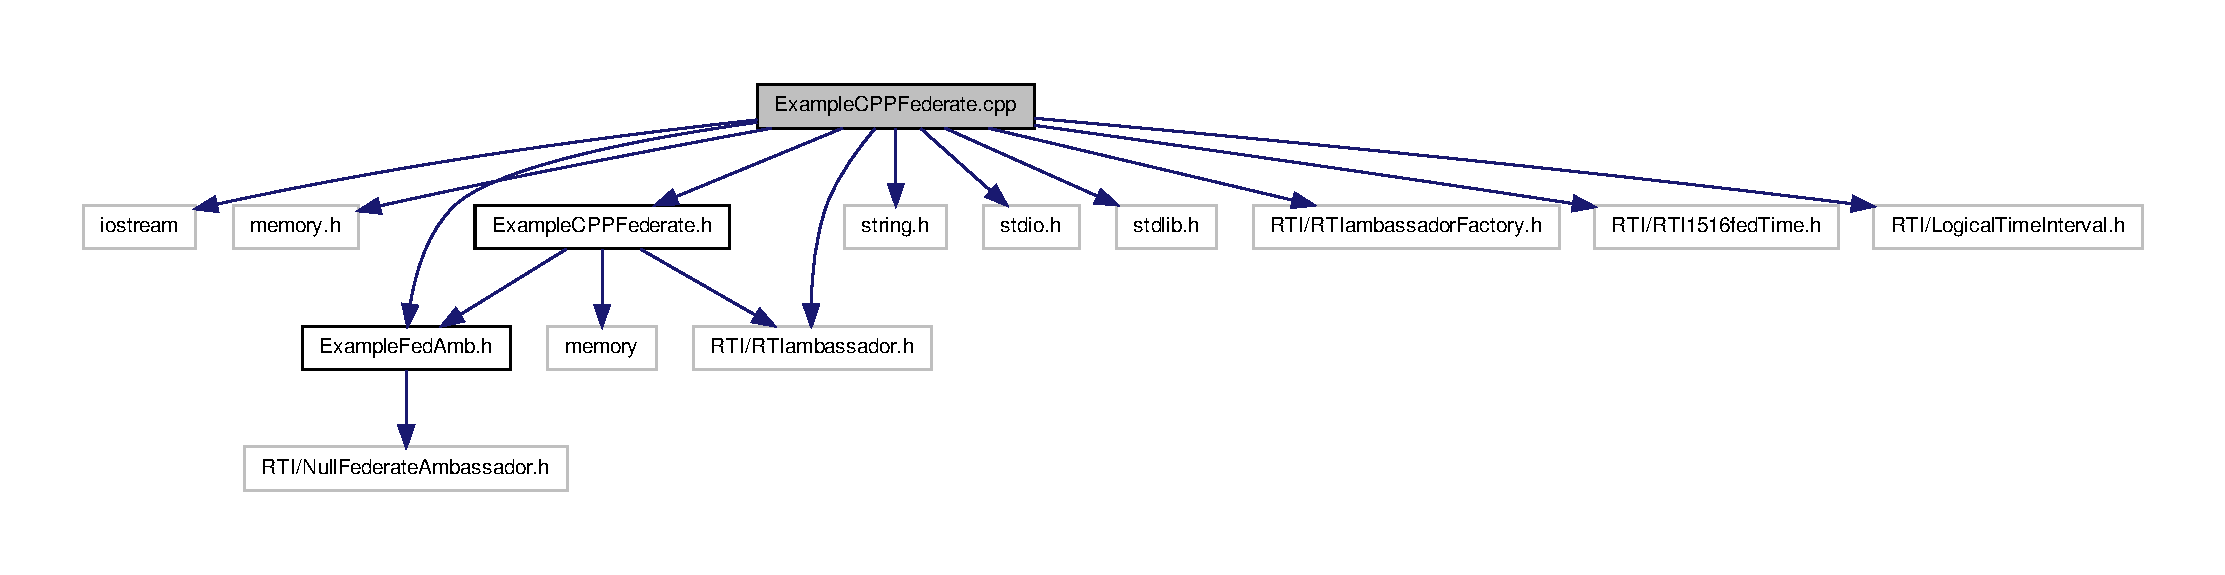
\includegraphics[width=400pt]{_example_c_p_p_federate_8cpp__incl}
\end{center}
\end{figure}


\subsection{Detailed Description}
Copyright (C) 2013 Max Oberberger $<$\href{mailto:max@oberbergers.de}{\tt max@oberbergers.de}$>$

Last modified: 2013 February 23, 20:05:02 by max

This file is part of ba-\/hla.

ba-\/hla is free software: you can redistribute it and/or modify it under the terms of the GNU General Public License as published by the Free Software Foundation, either version 3 of the License, or (at your option) any later version.

ba-\/hla is distributed in the hope that it will be useful, but WITHOUT ANY WARRANTY; without even the implied warranty of MERCHANTABILITY or FITNESS FOR A PARTICULAR PURPOSE. See the GNU General Public License for more details.

You should have received a copy of the GNU General Public License along with ba-\/hla. If not, see $<$\href{http://www.gnu.org/licenses/}{\tt http://www.gnu.org/licenses/}$>$. 
\hypertarget{_example_c_p_p_federate_8h}{
\section{ExampleCPPFederate.h File Reference}
\label{_example_c_p_p_federate_8h}\index{ExampleCPPFederate.h@{ExampleCPPFederate.h}}
}
{\ttfamily \#include \char`\"{}ExampleFedAmb.h\char`\"{}}\par
{\ttfamily \#include $<$RTI/RTIambassador.h$>$}\par
{\ttfamily \#include $<$memory$>$}\par
Include dependency graph for ExampleCPPFederate.h:\nopagebreak
\begin{figure}[H]
\begin{center}
\leavevmode
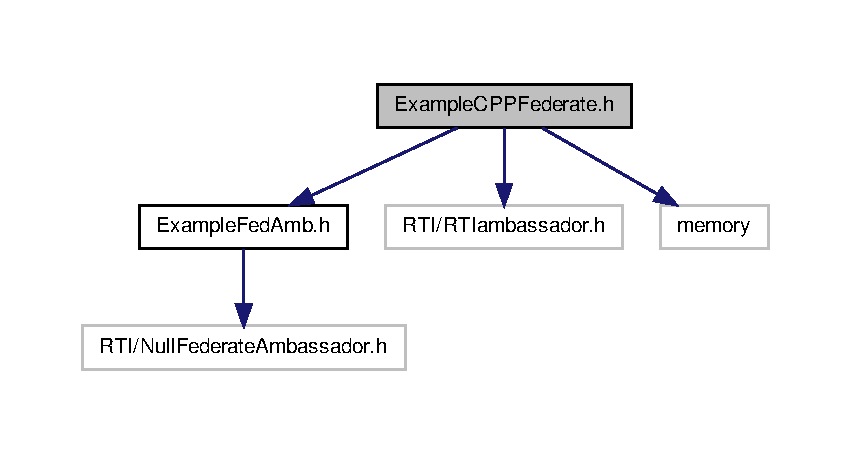
\includegraphics[width=400pt]{_example_c_p_p_federate_8h__incl}
\end{center}
\end{figure}
This graph shows which files directly or indirectly include this file:
\nopagebreak
\begin{figure}[H]
\begin{center}
\leavevmode
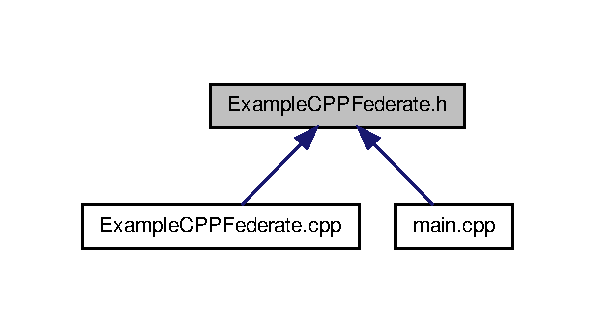
\includegraphics[width=286pt]{_example_c_p_p_federate_8h__dep__incl}
\end{center}
\end{figure}
\subsection*{Classes}
\begin{DoxyCompactItemize}
\item 
class \hyperlink{class_example_c_p_p_federate}{ExampleCPPFederate}
\end{DoxyCompactItemize}
\subsection*{Defines}
\begin{DoxyCompactItemize}
\item 
\hypertarget{_example_c_p_p_federate_8h_a2f5d7d447e5c7fa7586264f7713300ea}{
\#define {\bfseries READY\_\-TO\_\-RUN}~\char`\"{}ReadyToRun\char`\"{}}
\label{_example_c_p_p_federate_8h_a2f5d7d447e5c7fa7586264f7713300ea}

\end{DoxyCompactItemize}


\subsection{Detailed Description}
Copyright (C) 2013 Max Oberberger $<$\href{mailto:max@oberbergers.de}{\tt max@oberbergers.de}$>$

Last modified: 2013 February 23, 20:05:02 by max

This file is part of ba-\/hla.

ba-\/hla is free software: you can redistribute it and/or modify it under the terms of the GNU General Public License as published by the Free Software Foundation, either version 3 of the License, or (at your option) any later version.

ba-\/hla is distributed in the hope that it will be useful, but WITHOUT ANY WARRANTY; without even the implied warranty of MERCHANTABILITY or FITNESS FOR A PARTICULAR PURPOSE. See the GNU General Public License for more details.

You should have received a copy of the GNU General Public License along with ba-\/hla. If not, see $<$\href{http://www.gnu.org/licenses/}{\tt http://www.gnu.org/licenses/}$>$. 
\hypertarget{_example_fed_amb_8cpp}{
\section{ExampleFedAmb.cpp File Reference}
\label{_example_fed_amb_8cpp}\index{ExampleFedAmb.cpp@{ExampleFedAmb.cpp}}
}
{\ttfamily \#include $<$iostream$>$}\par
{\ttfamily \#include \char`\"{}ExampleFedAmb.h\char`\"{}}\par
{\ttfamily \#include $<$string.h$>$}\par
{\ttfamily \#include $<$RTI/RTI1516fedTime.h$>$}\par
Include dependency graph for ExampleFedAmb.cpp:\nopagebreak
\begin{figure}[H]
\begin{center}
\leavevmode
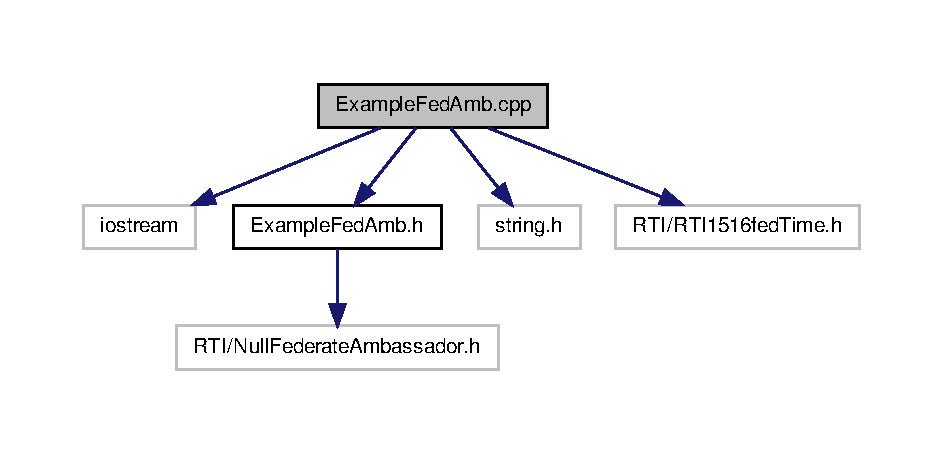
\includegraphics[width=400pt]{_example_fed_amb_8cpp__incl}
\end{center}
\end{figure}


\subsection{Detailed Description}
Copyright (C) 2013 Max Oberberger $<$\href{mailto:max@oberbergers.de}{\tt max@oberbergers.de}$>$

Last modified: 2013 February 23, 20:05:02 by max

This file is part of ba-\/hla.

ba-\/hla is free software: you can redistribute it and/or modify it under the terms of the GNU General Public License as published by the Free Software Foundation, either version 3 of the License, or (at your option) any later version.

ba-\/hla is distributed in the hope that it will be useful, but WITHOUT ANY WARRANTY; without even the implied warranty of MERCHANTABILITY or FITNESS FOR A PARTICULAR PURPOSE. See the GNU General Public License for more details.

You should have received a copy of the GNU General Public License along with ba-\/hla. If not, see $<$\href{http://www.gnu.org/licenses/}{\tt http://www.gnu.org/licenses/}$>$. 
\hypertarget{_example_fed_amb_8h}{
\section{ExampleFedAmb.h File Reference}
\label{_example_fed_amb_8h}\index{ExampleFedAmb.h@{ExampleFedAmb.h}}
}
{\ttfamily \#include $<$RTI/NullFederateAmbassador.h$>$}\par
Include dependency graph for ExampleFedAmb.h:\nopagebreak
\begin{figure}[H]
\begin{center}
\leavevmode
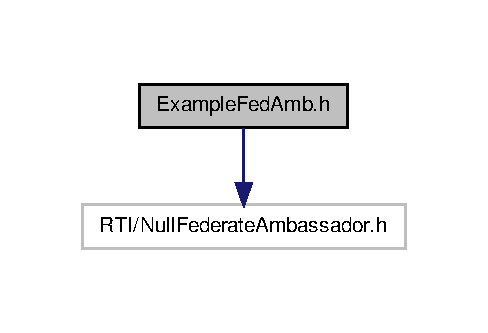
\includegraphics[width=234pt]{_example_fed_amb_8h__incl}
\end{center}
\end{figure}
This graph shows which files directly or indirectly include this file:
\nopagebreak
\begin{figure}[H]
\begin{center}
\leavevmode
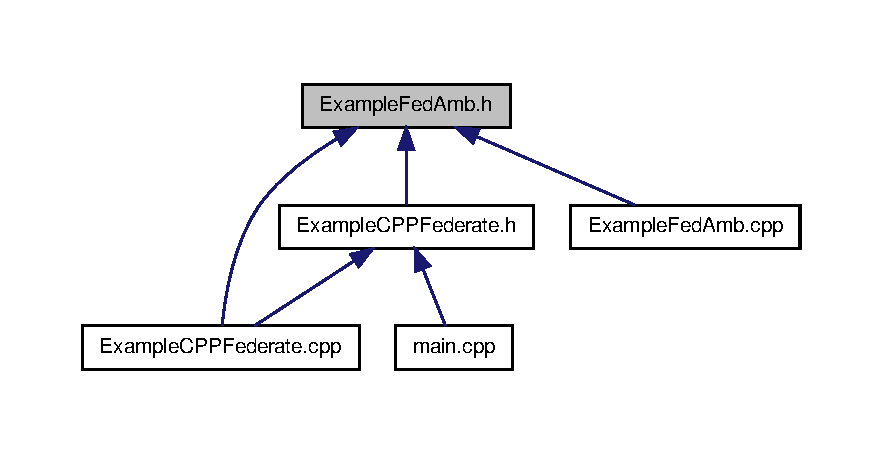
\includegraphics[width=400pt]{_example_fed_amb_8h__dep__incl}
\end{center}
\end{figure}
\subsection*{Classes}
\begin{DoxyCompactItemize}
\item 
class \hyperlink{class_example_fed_amb}{ExampleFedAmb}
\end{DoxyCompactItemize}


\subsection{Detailed Description}
Copyright (C) 2013 Max Oberberger $<$\href{mailto:max@oberbergers.de}{\tt max@oberbergers.de}$>$

Last modified: 2013 February 23, 20:05:02 by max

This file is part of ba-\/hla.

ba-\/hla is free software: you can redistribute it and/or modify it under the terms of the GNU General Public License as published by the Free Software Foundation, either version 3 of the License, or (at your option) any later version.

ba-\/hla is distributed in the hope that it will be useful, but WITHOUT ANY WARRANTY; without even the implied warranty of MERCHANTABILITY or FITNESS FOR A PARTICULAR PURPOSE. See the GNU General Public License for more details.

You should have received a copy of the GNU General Public License along with ba-\/hla. If not, see $<$\href{http://www.gnu.org/licenses/}{\tt http://www.gnu.org/licenses/}$>$. 
\hypertarget{main_8cpp}{
\section{main.cpp File Reference}
\label{main_8cpp}\index{main.cpp@{main.cpp}}
}
{\ttfamily \#include \char`\"{}ExampleCPPFederate.h\char`\"{}}\par
{\ttfamily \#include $<$stdio.h$>$}\par
{\ttfamily \#include $<$stdlib.h$>$}\par
{\ttfamily \#include $<$string.h$>$}\par
Include dependency graph for main.cpp:
\nopagebreak
\begin{figure}[H]
\begin{center}
\leavevmode
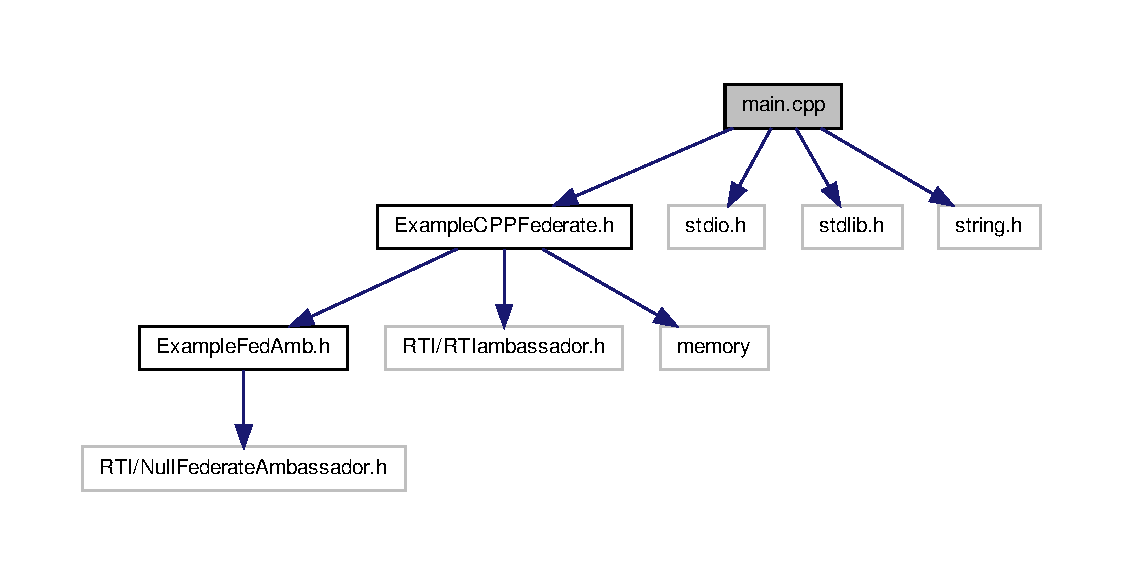
\includegraphics[width=400pt]{main_8cpp__incl}
\end{center}
\end{figure}
\subsection*{Functions}
\begin{DoxyCompactItemize}
\item 
\hypertarget{main_8cpp_a862cf0fce76408d4ac89d2ce51068f4f}{
void {\bfseries helpmenu} ()}
\label{main_8cpp_a862cf0fce76408d4ac89d2ce51068f4f}

\item 
\hypertarget{main_8cpp_a0ddf1224851353fc92bfbff6f499fa97}{
int {\bfseries main} (int argc, char $\ast$argv\mbox{[}$\,$\mbox{]})}
\label{main_8cpp_a0ddf1224851353fc92bfbff6f499fa97}

\end{DoxyCompactItemize}


\subsection{Detailed Description}
Copyright (C) 2013 Max Oberberger $<$\href{mailto:max@oberbergers.de}{\tt max@oberbergers.de}$>$

Last modified: 2013 February 23, 20:05:02 by max

This file is part of ba-\/hla.

ba-\/hla is free software: you can redistribute it and/or modify it under the terms of the GNU General Public License as published by the Free Software Foundation, either version 3 of the License, or (at your option) any later version.

ba-\/hla is distributed in the hope that it will be useful, but WITHOUT ANY WARRANTY; without even the implied warranty of MERCHANTABILITY or FITNESS FOR A PARTICULAR PURPOSE. See the GNU General Public License for more details.

You should have received a copy of the GNU General Public License along with ba-\/hla. If not, see $<$\href{http://www.gnu.org/licenses/}{\tt http://www.gnu.org/licenses/}$>$. 
\printindex
\end{document}
